\documentclass[dvipdfmx,11pt,notheorems]{beamer}
%%%% 和文用 %%%%%
\usepackage{bxdpx-beamer}
\usepackage{pxjahyper}
\usepackage{minijs}%和文用
\usepackage{listings,jlisting} % プログラムの表示用
\usepackage{type1cm}
\renewcommand{\kanjifamilydefault}{\gtdefault}%和文用

%%%% スライドの見た目 %%%%%
\usetheme{Boadilla}
\usecolortheme{seahorse}
\usefonttheme{professionalfonts}
\setbeamertemplate{frametitle}[default][center]
\setbeamertemplate{navigation symbols}{}
\setbeamercovered{transparent}%好みに応じてどうぞ)
\setbeamertemplate{footline}[page number]
\setbeamerfont{footline}{size=\normalsize,series=\bfseries}
\setbeamercolor{footline}{fg=black,bg=black}

\setbeamercolor{white-cyan1}
{fg=white,bg=cyan!80!black}
\setbeamercolor{white-cyan2}
{fg=white,bg=cyan!60!black}

%フラットデザイン化
\setbeamertemplate{blocks}[rounded] % Blockの影を消す
%Beamer色設定
\definecolor{UniBlue}{RGB}{0,150,200}
\definecolor{AlertOrange}{RGB}{255,76,0}
\definecolor{AlmostBlack}{RGB}{38,38,38}
\setbeamercolor{structure}{fg=UniBlue} % 見出しカラー
\setbeamercolor{block title}{fg=UniBlue!50!black} % ブロック部分タイトルカラー
%%%%

%%%% 定義環境 %%%%%
\usepackage{amsmath,amssymb}
\usepackage{amsthm}
\usepackage{bm}
\theoremstyle{definition}
\newtheorem{theorem}{定理}
\newtheorem{definition}{定義}
\newtheorem{proposition}{命題}
\newtheorem{lemma}{補題}
\newtheorem{corollary}{系}
\newtheorem{conjecture}{予想}
\newtheorem*{remark}{Remark}
\renewcommand{\proofname}{}
%%%%%%%%%

%%%%% フォント基本設定 %%%%%
% \usepackage[T1]{fontenc}%8bit フォント
% \usepackage{textcomp}%欧文フォントの追加
% \usepackage[utf8]{inputenc}%文字コードをUTF-8
% \usepackage{otf}%otfパッケージ
% \usepackage{lxfonts}%数式・英文ローマン体を Lxfont にする
% \usepackage{bm}%数式太字
%%%%%%%%%%

%%%%% 複数人の著者を揃える %%%%%
%% http://tex.stackexchange.com/questions/
%%   166531/how-to-change-author-alignment-in-beamer
\makeatletter
\long\def\beamer@author[#1]#2{%
  \def\insertauthor{\def\inst{\beamer@insttitle}\def\and{\beamer@andtitle}%
  \begin{tabular}{rl}#2\end{tabular}}%
  \def\beamer@shortauthor{#1}%
  \ifbeamer@autopdfinfo%
    \def\beamer@andstripped{}%
    \beamer@stripands#1 \and\relax
    {\let\inst=\@gobble\let\thanks=\@gobble\def\and{, }\hypersetup{pdfauthor={\beamer@andstripped}}}
  \fi%
}
\makeatother
%%%%%%%%%%

%%%%% プログラムに色をつける
\usepackage{color}

\definecolor{codegreen}{rgb}{0,0.6,0}
\definecolor{codegray}{rgb}{0.5,0.5,0.5}
\definecolor{codepurple}{rgb}{0.58,0,0.82}
\definecolor{backcolour}{rgb}{0.95,0.95,0.92}

\lstdefinestyle{mystyle}{
    backgroundcolor=\color{backcolour},
    commentstyle=\color{codegreen},
    keywordstyle=\color{magenta},
    numberstyle=\tiny\color{codegray},
    stringstyle=\color{codepurple},
    basicstyle=\footnotesize,
    breakatwhitespace=false,
    breaklines=true,
    captionpos=b,
    keepspaces=true,
    numbers=left,
    numbersep=5pt,
    showspaces=false,
    showstringspaces=false,
    showtabs=false,
    tabsize=2
}

\lstset{style=mystyle}

%%%%
\title[略タイトル]{第9回 知能システム学特論レポート}%[略タイトル]{タイトル}
\author[NishidaLab]{
15344203 & 有田 裕太 \\
15344206 & 緒形 裕太 \\
15344209 & 株丹 亮 \\
12104125 & 宮本 和 }%[略名前]{名前}
\institute[NishidaLab]{西田研究室,計算力学研究室}%[略所属]{所属}
\date{2015年\ 7月\ 16日}%日付

\begin{document}

%%%% 1 %%%%
\begin{frame}[plain]\frametitle{}
\titlepage %表紙
\end{frame}

% \begin{frame}\frametitle{Contents}
% \tableofcontents %目次
% \end{frame}

%%%% 進捗状況 %%%%
\begin{frame}\frametitle{進捗状況}

\begin{block}{理論研究の進捗}
畳込みニューラルネットワークの理論について
\end{block}

\vspace{1cm}
\begin{exampleblock}{プログラミングの進捗}
学習器のパラメータ設定について\\
データセットを作成し,学習を行った結果
\end{exampleblock}
\end{frame}

%%%% 局所コントラスト正規化%%%%
\begin{frame}[fragile]\frametitle{局所コントラスト正規化}

 \begin{block}{局所コントラスト正規化}
 画像の中から対象物を捉えるための、画像の濃淡を正規化する方法の一種
 \end{block}

 \begin{itemize}
  \item 1つの層だけでこの処理が可能
  \item 畳み込みネットに組み込むことが可能
  \item 層の重みは固定され,学習の対象となるパラメータはない
  \item 減算正規化と除算正規化の2種類がある

 \end{itemize}
\end{frame}

 %%%% ogata %%%%
\begin{frame}[fragile]\frametitle{減算正規化}
 \begin{block}{減算正規化}
入力画像の各画素濃淡から平均を差し引く
 \begin{equation}
 z_{ij} = x_{ij}-\bar{x}_{ij}
 \end{equation}
 \end{block}
濃淡値の平均
 \begin{equation}
 \bar{x}_{ij}= \sum_{(p,q)\in{P_{ij}}}^{} x_{i+p,j+q}
 \end{equation}

 \begin{itemize}
 \item $i,j$:入力画像の画素
 \item $p,q$:フィルタの画素
 \end{itemize}
\end{frame}

\begin{frame}[fragile]\frametitle{除算正規化}
 \begin{block}{除算正規化}
同じ局所領域内で画素値の分散を抑える
 \begin{equation}
 z_{ij}=\frac{x_{ij}-\bar{x}_{ij}}{\sigma_{ij}}
 \end{equation}
 \end{block}
画素値の分散
 \begin{equation}
 \sigma^2_{ij}=\sum_{(p,q)\in{P_{ij}}}^{} w_{pq}(x_{i+p,j+q}-\bar{x}_{ij})^2
 \end{equation}

 \begin{itemize}
 \item $w_{pq}$:重み
 \end{itemize}

\end{frame}

\begin{frame}[fragile]\frametitle{除算正規化}
以上の計算をそのまま行うと,濃淡変化が少ない局所領域ほど濃淡変化が増幅され,
ノイズが強調される.そこで,入力画像のコントラストが大きい部分にのみ適用
するため,ある定数$c$を設定し濃淡の標準偏差がこれを下回る
($\sigma_{ij}<c$)で除算する
\begin{equation}
 z_{ij}=\frac{x_{ij}-\bar{x}_{ij}}{max(\sigma_{ij}<c)}
\end{equation}
や,同様の効果が$\sigma_{ij}$に応じて連続的に変化する
\begin{equation}
 z_{ij}=\frac{x_{ij}-\bar{x}_{ij}}{\sqrt{\sigma_{ij}+c}}
\end{equation}
を用いる.
\end{frame}

% %%%% プーリング 1 %%%%
% \begin{frame}[fragile]\frametitle{プーリング}
% \begin{block}{プーリング}
% プーリング層は通常,畳み込み層の直後に設置され,プーリング層は畳み込み層で抽出された特徴の位置
% 感度を低下させる働きがある.
% \end{block}
% サイズ$W \times W \times K$の入力画像上で画素$(i,j)$を中心とする$H\times H$の正方領域とり,この中に含まれる画素の集合を$P_{ij}$で表す.$P_{ij}$内の画素についてチャネル$k$ごとに独立に,$H^2$個ある画素値を使って1つの画素値$u_{ijk}$を求める.

% \begin{itemize}
%  \item 最大プーリング(max pooling)
% 	   \begin{eqnarray}
% 		u_{ijk} = \max_{(p,q) \in P_{ij}} z_{pqk}
% 	   \end{eqnarray}
%  \item 平均プーリング(average pooling)
% 	   \begin{eqnarray}
% 		u_{ijk} = \frac{1}{H^{2}}\sum_{(p,q) \in P_{ij}} z_{pq}
% 	   \end{eqnarray}

% \end{itemize}

% \end{frame}

% %%%% 学習パラメータの設定 1 %%%%
\begin{frame}[fragile]\frametitle{学習パラメータの設定}
学習を行う上で必要なパラメータについて説明する.\\この設定が記述されているファイルはcifar10\_quick\_solver.prototxtである.

\begin{lstlisting}[basicstyle=\ttfamily\footnotesize, frame=single, firstnumber=1, numbers=left, breaklines=true]
net: "examples/cifar10/cifar10_quick_train_test.prototxt"
test_iter: 100
test_interval: 500
base_lr: 0.0001
momentum: 0.9
weight_decay: 0.004
lr_policy: "fixed"
display: 100
max_iter: 4000
snapshot: 4000
snapshot_prefix: "examples/cifar10/cifar10_quick"
solver_mode: GPU
\end{lstlisting}
\begin{exampleblock}{単位[batch]の定義}
教師データを一度にいくつ処理するか(バッチサイズ)を決定し,これを1[batch]とする.
\end{exampleblock}
\end{frame}

% %%%% 学習パラメータの設定 2 %%%%
\begin{frame}[fragile]\frametitle{学習パラメータの設定}
各項目の意味を以下に示す.
\begin{description}
  \item[net :]学習用ネットワーク定義ファイルを指定する.
  \item[test\_iter :]学習中の正答率評価を1回行うのに使う評価セットの\\データ数をバッチ数で指定.
  \item[test\_interval :]テストデータから正答率評価を行う間隔をバッチ数で指定.
  \item[base\_lr,\ momentum,\ weight\_decay,\ lr\_policy :]学習率に関する設定.
  \item[display :]学習中のステータスを出力する回数をバッチ数で指定.
  \item[max\_iter :]学習の計算を最大どれだけ続けるかを訓練データの\\バッチ数で指定.
  \item[snapshot,\ snapshot\_prefix :]学習の途中経過を保存する間隔と場所を指定.
  \item[solver\_mode :]学習をCPUのみ,あるいはGPUを用いるかを指定.
\end{description}
\end{frame}



%%%% Caffeで学習を行うまでの流れ %%%%
\begin{frame}\frametitle{学習データの用意}
\begin{figure}[t]
 \begin{minipage}{0.2\hsize}
  \centering
  \text{eri} \\
  \centering
  
\includegraphics[width=20mm,bb=0 0 200 200]{./fig/png/faces/eri.png} \\
  \text{1908枚}
 \end{minipage}
 \begin{minipage}{0.2\hsize}
  \centering
  \text{hanayo} \\
  \centering
  
\includegraphics[width=20mm,bb=0 0 200 200]{./fig/png/faces/hanayo.png}\\
  \text{2220枚}
 \end{minipage}
 \begin{minipage}{0.2\hsize}
  \centering
  \text{honoka} \\
  \centering
  
\includegraphics[width=20mm,bb=0 0 200 200]{./fig/png/faces/honoka.png}\\
  \text{2733枚}
 \end{minipage}
 \begin{minipage}{0.2\hsize}
  \centering
  \text{kotori} \\
  \centering
  
\includegraphics[width=20mm,bb=0 0 200 200]{./fig/png/faces/kotori.png}\\
  \text{1722枚}
 \end{minipage}
\end{figure}
\begin{figure}[t]
 \begin{minipage}{0.17\hsize}
  \centering
  \text{maki} \\
  \centering
  
\includegraphics[width=20mm,bb=0 0 200 200]{./fig/png/faces/maki.png}\\
  \text{1874枚}
 \end{minipage}
 \begin{minipage}{0.17\hsize}
  \centering
  \text{niko} \\
  \centering
  
\includegraphics[width=20mm,bb=0 0 200 200]{./fig/png/faces/niko.png}\\
  \text{1910枚}
 \end{minipage}
 \begin{minipage}{0.17\hsize}
  \centering
  \text{nozomi} \\
  \centering
  
\includegraphics[width=20mm,bb=0 0 200 200]{./fig/png/faces/nozomi.png}\\
  \text{1489枚}
 \end{minipage}
 \begin{minipage}{0.17\hsize}
  \centering
  \text{rin} \\
  \centering
  
\includegraphics[width=20mm,bb=0 0 200 200]{./fig/png/faces/rin.png} \\
  \text{2425枚}
 \end{minipage}
 \begin{minipage}{0.17\hsize}
  \centering
  \text{umi} \\
  \centering
  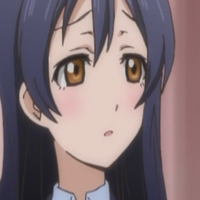
\includegraphics[width=20mm,bb=0 0 200 200]{./fig/png/faces/umi.png}\\
  \text{1703枚}
 \end{minipage}
 \end{figure}
他に負例(etc)として7001枚の画像($200\times200\times3$)を用意
\end{frame}

\begin{frame}[fragile]\frametitle{学習}
 今回はネットワークモデルにcifar10のモデルを用いて学習を行った.
\begin{lstlisting}[basicstyle=\ttfamily\footnotesize, frame=single, tabsize=2,showtabs,firstnumber=1, numbers=left, breaklines=true]
build/tools/caffe train --solver examples/cifar10/cifar10_quick_solver.prototxt
\end{lstlisting}
\begin{exampleblock}{cifar10\_quick.prototxt}
 畳込み層3層,プーリング層3層,全結合層2層,活性化関数はSoftmax関数を用いている.
\end{exampleblock}
\begin{itemize}
 \item test\_iter : 100
 \item max\_iter : 4000
 \item batch\_size : 100
 \item solver\_mode : CPU
\end{itemize}
\end{frame}

\begin{frame}[fragile]\frametitle{学習結果}
\begin{figure}[ht]
 \centering
 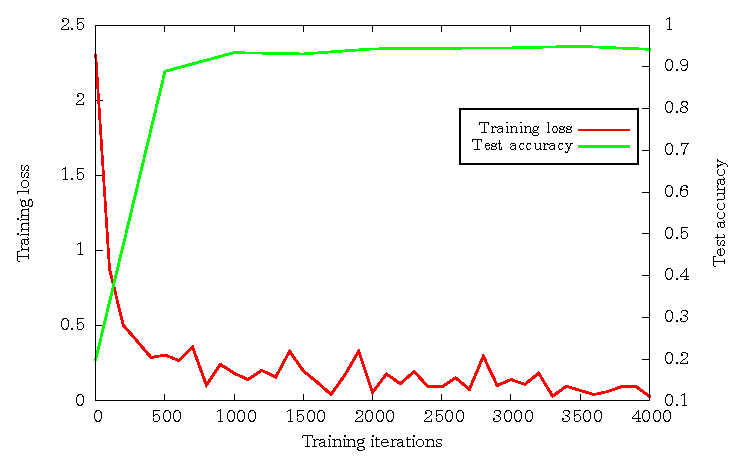
\includegraphics[scale=1.0]{fig/eps/result_train_test_graph.eps}
 \caption{損失関数の値と精度 }
\end{figure}

\end{frame}
%%%% 今後の課題 %%%%
\begin{frame}\frametitle{今後の課題}

\begin{block}{理論研究}
CNNの詳細な調査
\end{block}

\vspace{1cm}
\begin{exampleblock}{プログラミング}
学習によって得られた識別器を用いて実際に識別してみる
\end{exampleblock}
\end{frame}

% \begin{figure}[t]
%  \begin{minipage}{0.3\hsize}
%   \centering
%   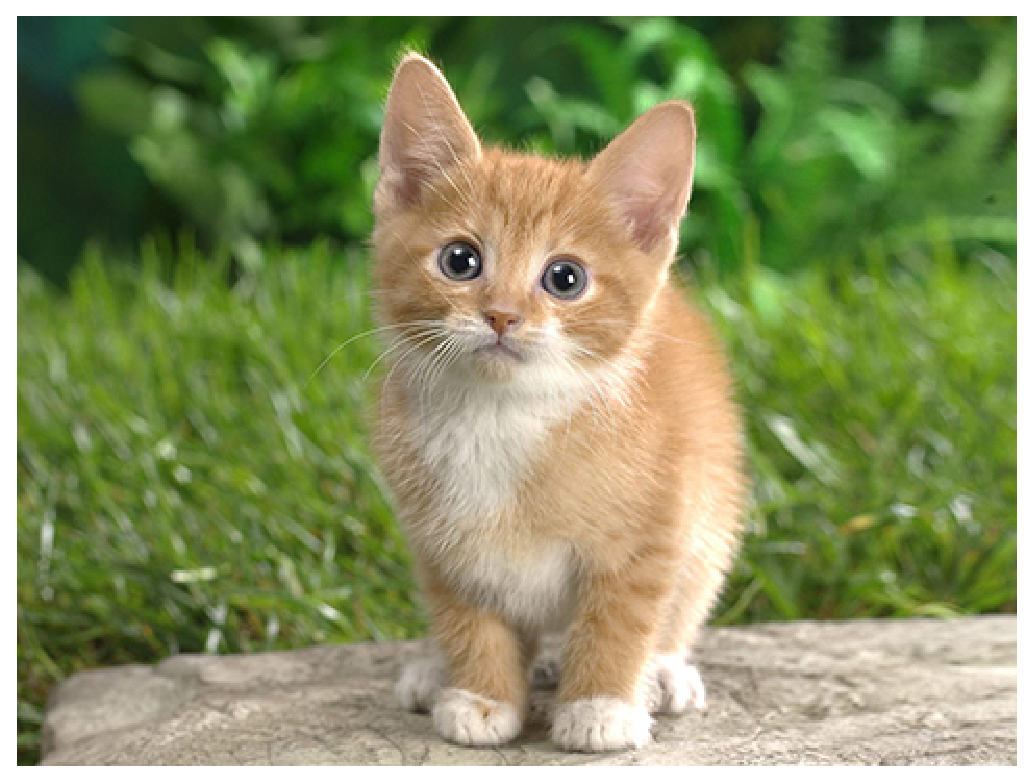
\includegraphics[width=30mm]{./figure/cat.eps}
%   \caption{cat.jpg}
%   \label{sample1}
%  \end{minipage}
%  \begin{minipage}{0.3\hsize}
%   \centering
%   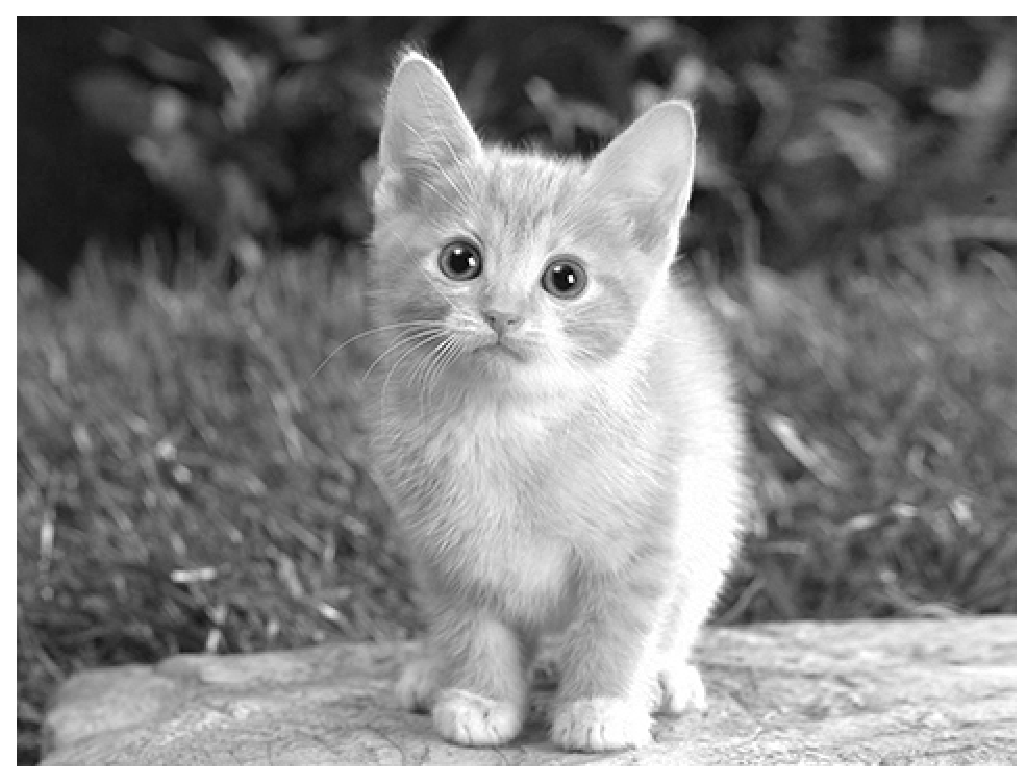
\includegraphics[width=30mm]{./figure/cat_gray.eps}
%   \caption{cat\_gray.jpg}
%   \label{sample2}
%  \end{minipage}
%  \begin{minipage}{0.3\hsize}
%   \centering
%   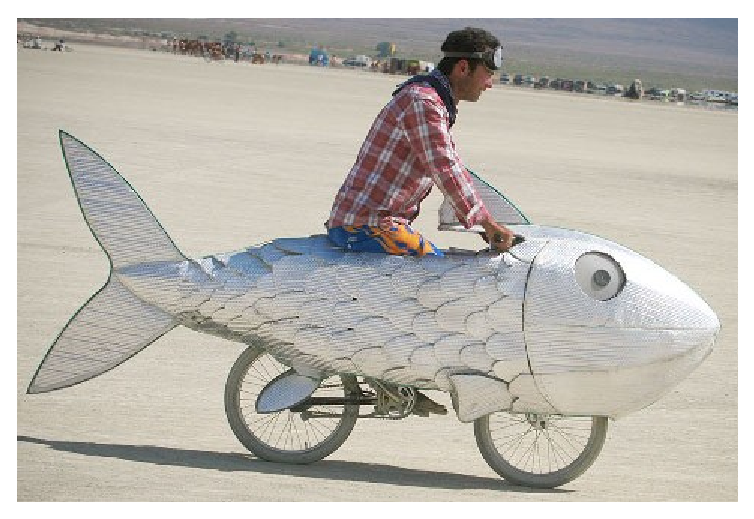
\includegraphics[width=30mm]{./figure/fish-bike.eps}
%   \caption{fish-bike.jpg}
%   \label{sample3}
%  \end{minipage}
% \end{figure}
% \begin{exampleblock}{実行環境}
% \begin{itemize}
%  \item Ubuntu 14.04 LTS
%  \item Intel core i5-4440 3.10GHz$\times$4
%  \item RAM 16GB
% \end{itemize}
% \end{exampleblock}
% \end{frame}


% \section{具体例}

% \begin{frame}\frametitle{定理環境の例}
% \begin{theorem}[Fermat]
% $a^{p-1} \equiv 1 \pmod{p}$
% \end{theorem}
% \pause
% \begin{theorem}[Wilson]
% \begin{equation}
% (p-1)! \equiv 1 \pmod{p}
% \end{equation}
% \end{theorem}
% \end{frame}

% \begin{frame}<1-2>\frametitle{オーバーレイ}
% \onslide*<1>{
% \Large{これは1枚目です}
% }
% \onslide*<2>{
% これは2枚目です
% \begin{theorem}[Euclid]
% There is no largest prime number.
% \end{theorem}
% }
% \end{frame}

% \begin{frame}\frametitle{色もつけれるよ}
%   {\color{red} red}(\alert{alert}),
%   {\color{blue} blue}(\structure{structure}),
%   {\color{green} green},
%   {\color{cyan} cyan},
%   {\color{magenta} magenta},
%   {\color{yellow} yellow},
%   {\color{black} black},
%   {\color{darkgray} darkgray},
%   {\color{gray} gray},
%   {\color{lightgray} lightgray},
%   {\color{orange} orange},
%   {\color{violet} violet},
%   {\color{purple} purple},
%   {\color{brown} brown},
% \end{frame}

% \begin{frame}\frametitle{いろんなブロック}
% \begin{block}{ブロック}
% これは普通のブロックです
% \end{block}

% \begin{alertblock}{警告ブロック}
% 警告!これは警告ブロックだ!
% \end{alertblock}

% \begin{exampleblock}{例ブロック}
% 例えば、こんなブロックです。
% \end{exampleblock}
% \end{frame}

% \begin{frame}<1-2>\frametitle{画像も貼れるよ}
% \onslide*<1>{
% このように画像を貼れるよ
% %\begin{figure}[htb]
% %\centering
% %\includegraphics[width=12cm,clip]{dummygraph.pdf}
% %\caption{$f(x)=e^{-\frac{x}{10}}\sin(x)$}
% %\end{figure}%
% }
% \onslide*<2>{
% 画像や表は各自用意してね
% %\begin{figure}[htb]
% %\centering
% %\includegraphics[width=8cm,clip]{sym4.pdf}
% %\caption{Cayley graph of $\mathfrak{S}_{4}$}
% %\end{figure}%
% }
% \end{frame}

% \begin{frame}\frametitle{まとめ}
% \LARGE{大事なのは中身です!}
% \end{frame}

% \begin{frame}\frametitle{}
% {\Large ありがとうございました}
% \end{frame}
% \appendix

\newcounter{finalframe}
\setcounter{finalframe}{\value{framenumber}}

% \begin{frame}[containsverbatim]\frametitle{dvipngの使い方(1)}
% \begin{block}{この様なファイルを用意する}
% \tiny{
% \begin{verbatim*}
% \documentclass[43pt]{jsarticle}
% \usepackage{amsmath}
% \usepackage{lmodern}
% \pagestyle{empty}
% \begin{document}
% \begin{equation*}
% \sum_{k=0}^{\infty} \frac{(2k)!}{2^{2k}(k!)^2} \frac{1}{2k+1}=\frac{\pi}{2}
% \end{equation*}
% \end{document}
% \end{verbatim*}
% }
% \end{block}
% \end{frame}

% \begin{frame}[containsverbatim]\frametitle{dvipngの使い方(2)}
% \begin{block}{使い方(コマンドライン)}
% \scriptsize{
% \begin{verbatim*}
% latex dvipng-sample.tex
% dvipng dvipng-sample.dvi -T tight -bd 1000
% \end{verbatim*}
% }
% \end{block}
% \end{frame}
\setcounter{framenumber}{\value{finalframe}}
\end{document}